\documentclass{beamer}
\PassOptionsToClass{handout}{beamer}


\usetheme{Madrid}

\usepackage{graphicx}
\usepackage{hyperref}
\usepackage{subcaption}
\usepackage{float}
\usepackage{csquotes}
\usepackage{pifont}
\setbeamertemplate{navigation symbols}{}
\usepackage[ngerman]{babel}
\usepackage[style=verbose,backend=bibtex]{biblatex}
\usepackage{algorithm2e}
\RestyleAlgo{ruled}

\setbeamertemplate{footline}
{
  \leavevmode%
  \hbox{%
  \begin{beamercolorbox}[wd=.333333\paperwidth,ht=2.25ex,dp=1ex,center]{author in head/foot}%
    \usebeamerfont{author in head/foot}Ian Schmetkamp%\insertshortauthor
  \end{beamercolorbox}%
  \begin{beamercolorbox}[wd=.333333\paperwidth,ht=2.25ex,dp=1ex,center]{title in head/foot}%
    \usebeamerfont{title in head/foot}Autonomous Object Inspection
  \end{beamercolorbox}%
  \begin{beamercolorbox}[wd=.333333\paperwidth,ht=2.25ex,dp=1ex,right]{date in head/foot}%
    \usebeamerfont{date in head/foot}\insertshortdate{}\hspace*{2em}
    \insertframenumber{} / \inserttotalframenumber\hspace*{2ex}
  \end{beamercolorbox}}%
  \vskip0pt%
}
\title{Autonomous Object Inspection with Mobile Robots for 3D Reconstruction and Image Data Acquisition}
\author{Ian Schmetkamp \inst{1} \\ \textbf{Advisor:} Philip Keller \inst{2} \\ \textbf{Supervisor:} Prof. Dr.-Ing. Rüdiger Dillmann \inst{2}}
\subtitle{Bachelor Thesis}
\institute{Karlsruhe Institute of Technology \and FZI Research Center for Information Technology}
\date{\today}

\begin{document}
\frame{\titlepage}
\frame{\frametitle{Inhalt}\tableofcontents}

\section{Allgemeines}
\begin{frame}{Aufgabe}
	\begin{minipage}{0.55 \textwidth}
		\begin{block}{Ziel}
			\begin{itemize}
				\item autonom Bilder von Object aufnehmen
				\item Bilder aus verschiedenen Perspektiven
				\item Roboter (Spot, Turtlebot, etc.) muss nächste, vorteilhafte Perspektive berechnen
			\end{itemize}
		\end{block}
	\end{minipage}
	\hfill
	\begin{minipage}{0.4 \textwidth}
		\centering
		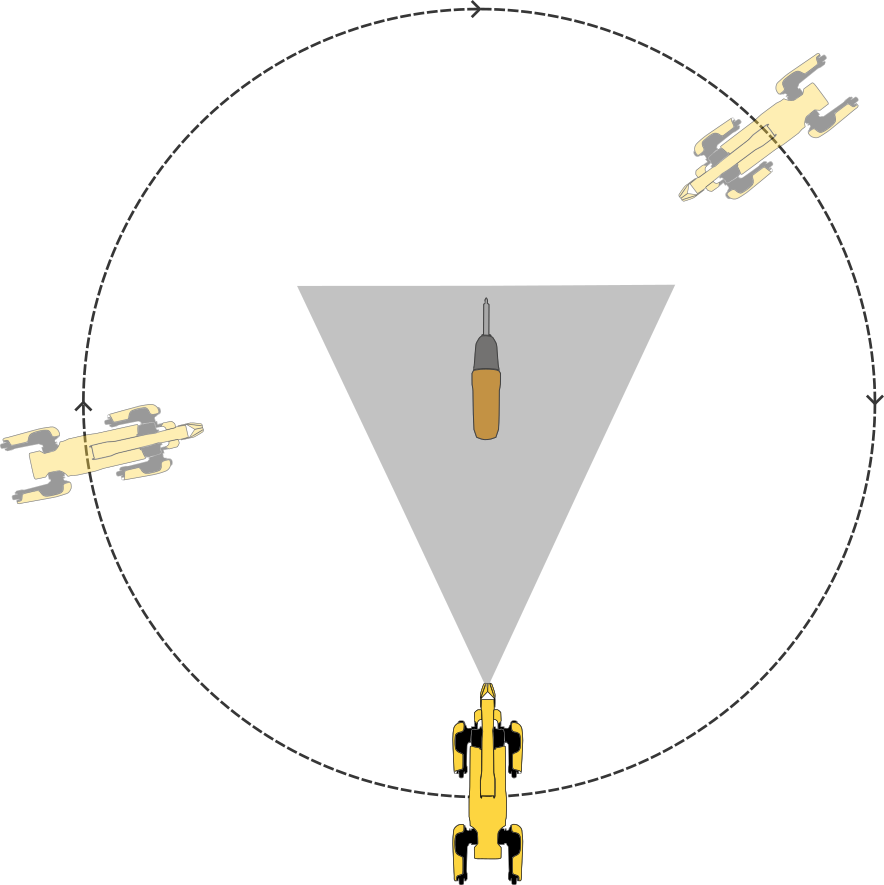
\includegraphics[width=1\textwidth]{Graphics/graphic_top_down.png}
	\end{minipage}
\end{frame}

\begin{frame}{Ansatz}
	\begin{block}{Ansatz}
		\begin{itemize}
			\item Mögliche Positionen evaluieren
			\item Abschätzen wie viel Informationen in möglicher Position gesehen wird (Stichwort: Next-Best-View)
			\item Andere Faktoren für Positionen evaluieren (Distanz, Überlappung, Sichtbarkeit des Bekannten etc.)
			\item Zur besten Position gehen
		\end{itemize}
	\end{block}
	\centering
	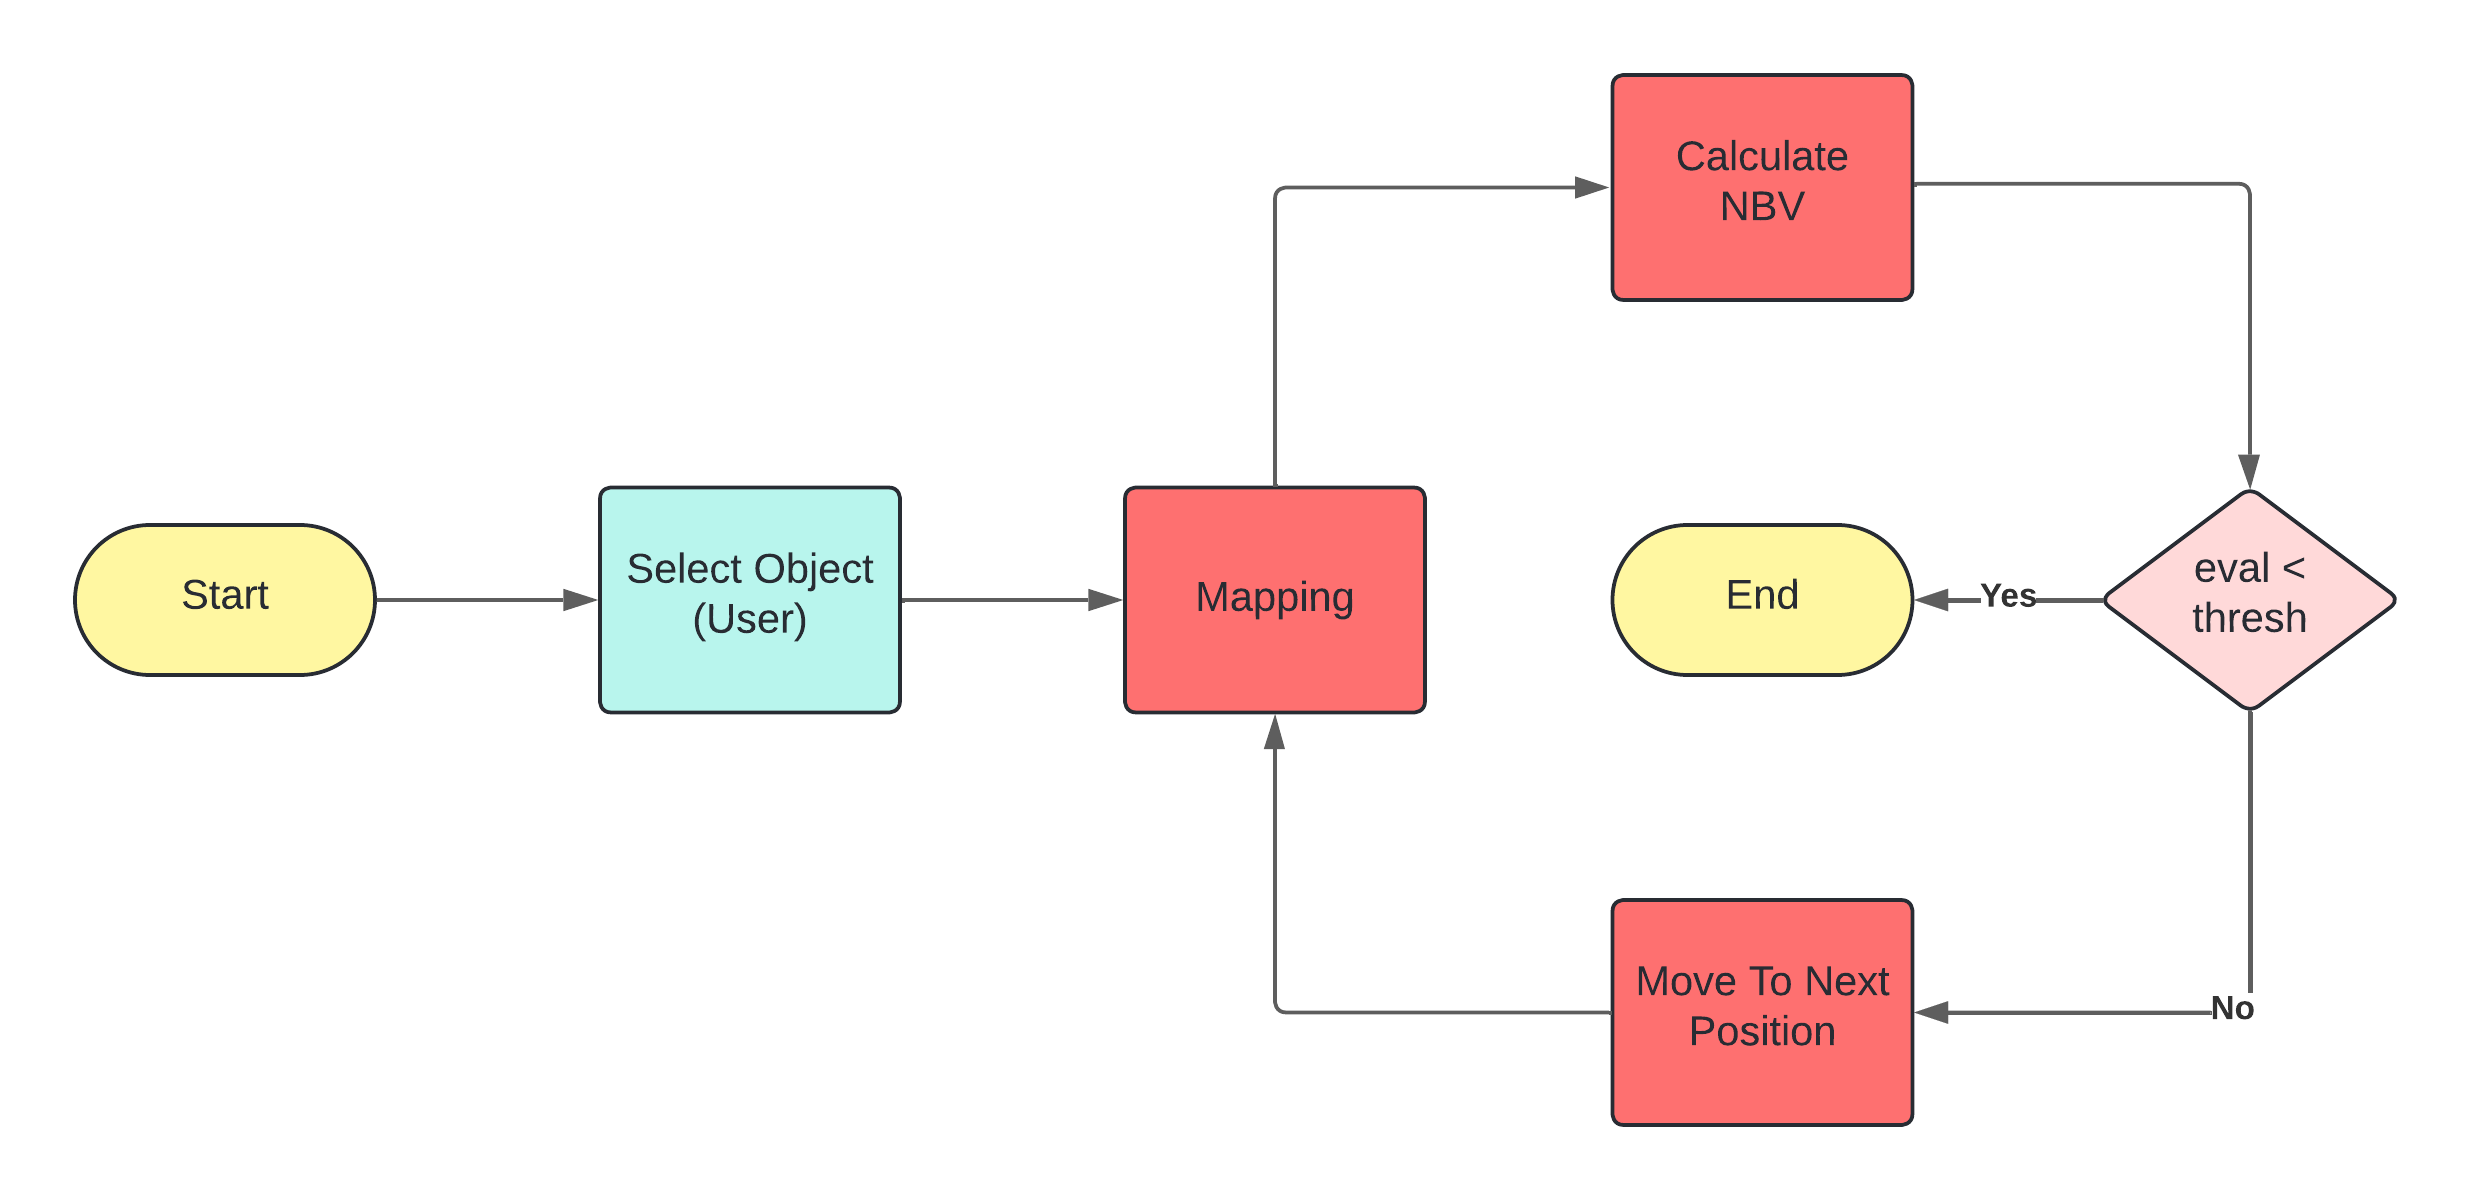
\includegraphics[width=0.9\textwidth]{Graphics/flow_chart.png}
\end{frame}

\section{Algorithmen}
\begin{frame}{Algorithmen}
	\begin{algorithm}
		\KwData{pixel_x, pixel_y: int}
		ray = convertPixelToRay(pixel_x, pixel_y)\;
		makeScan(), makeImage()\;
		origin = raytrace(camera.position, ray)\;
		\While{True}{
			occupied, frontier_voxel =  breadthFirstSearch(origin)\;
			frontiers = groupFrontiers(frontier_voxel)\;
		}
	\end{algorithm}
\end{frame}


\end{document}
